
\chapter{Scrubbing and motion artefact correction} 

\section{Introduction} Head motion is probably the most severe problem in fMRI studies, although it cannot be avoided. The quality of the fMRI data is strongly affected by the presence of head motion. As previously mention, a number of publications have proposed post-hoc correction in order to reduce head motion artefact. Although head motion can be corrected in the image space, displacement of the head reduces the homogeneity of the magnetic field, which is fine-tuned prior to functional scans for a given head position. Since head displacements lead to non-optimal tuning, motion artefacts are not fully removed even after perfect realignment of successive functional volumes in image space. The impact of motion and the method available to reduce its effect on functional connectivity thus need to be carefully evaluated. Typically subjects with average motion over 3 mm are excluded from the analysis. A first popular technique to reduce motion artifact is global signal correction (GSC), which consists of 
regressing the average of all the time-series in the brain. This 
technique has raised a number of concerns due to the potential artificial introduction of anti-correlation in the data \citep{Fox2009,Murphy2009, Saad2012, Carbonell2014, Power2014}. Another corrective measure is the CompCor method \citep{Behzadi2007} that regresses out the $n$ first components of a principal component analysis (PCA) on the time-series of the white matter and cerebrospinal fluids voxels. As no signal of neuronal origin are expected in such areas, the CompCor method was suggested to provide a compact representation of the structured noise present in an fMRI dataset. Both GSC and CompCor are global corrections, which are not specific to motion correction. The GSC in particular incorporates signal from the grey matter regions. Power and colleagues showed in 2012 that spurious but systematic correlations in fc-MRI arise from subject motion even at levels previously regarded as insignificant  (variation smaller than $1$ mm / degree in motion parameters) and are not adequately removed by common 
functional connectivity processing steps. \cite{Power2012} suggested using a method called ``scrubbing'' (or censoring) in order to reduce motion-related bias from  fMRI time-series. With the scrubbing method, the frames with motion level above a certain threshold are simply removed from the time-series. The metric used to quantify the level of motion from one frame to the other is called framewise displacement (FD). It is calculated as the sum of the absolute values of the differentiated realignment parameters estimated at every time point, giving an approximate conversion of rotation parameters ($\alpha_{i},\beta_{i},\gamma_{i}$) in a unit equivalent to a translation in millimeters on a sphere of radius 50mm and translation parameters ($d_{ix},d_{iy},d_{iz}$) for the other rigid body parameters.
The main limitation of the scrubbing method is the loss of time-points, which can lead to subjects loss due to an insufficient number of time point remaining after scrubbing correction. The question is therefore to evaluate if the trade-off between data loss and quality is detrimental or beneficial to statistical power. I have recently published results concerning this issue \cite{Dansereau2014} (published proceeding and manuscript in preparation). In this work we aimed to (1) characterize the impact of motion on rs-fMRI in cognitively normal elderly (CNE)  participants as well as patients with mild cognitive impairment (pMCI) and dementia of the Alzheimer's type 0.5-No (pDAT), and, (2) evaluate how the scrubbing impacts the differences in connectivity between groups (CNE, pMCI, pDAT).

\begin{equation}\label{Frame displacement} 
  \triangle d_{ix} = d_{(i-1)x} - d_{ix}\text{, derivative of a translation parameter in the x axis}
\end{equation}

\begin{equation}\label{Frame displacement}  
    FD_{i} = \vert \triangle d_{ix} \vert + \vert \triangle d_{iy} \vert + \vert \triangle d_{iz} \vert + \vert \triangle \alpha_{i} \vert + \vert \triangle \beta_{i} \vert + \vert \triangle \gamma_{i} \vert.  
\end{equation}

\section{Method}
\subsection{Dataset}
This project was based on a real dataset with fMRI data acuquired in different settings. The dataset included 313 elderly adults agregated across 5 independent studies: the ADNI2 study and 4 other studies based in Montreal, Canada. The dataset included three different clinical cohorts, for a grand total of 126 CNE participants (51 males, age range = 57-94 yrs), 133 patients with MCI (70 males, age range = 55-89 yrs), and 54 patients with DAT (22 males, age range = 55-88 yrs). We also included 355 cognitively normal young adults (CNY) from the 1000 functional connectome project (150 males, age range = 18-46 yrs) as a reference dataset \citep{Biswal2010}. This project was approved by the local ethics review board. 

\subsection{Preprocessing}
The datasets were analysed using the NeuroImaging Analysis Kit (NIAK\footnote{\url{http://www.nitrc.org/projects/niak/}}) version 0.12.14, under CentOS version 6.3 with Octave\footnote{\url{http://gnu.octave.org}} version 3.8.1 and the Minc toolkit\footnote{\url{http://www.bic.mni.mcgill.ca/ServicesSoftware/ServicesSoftwareMincToolKit}} version 0.3.18. Analyses were executed in parallel on the "Mammouth" supercomputer\footnote{\url{http://www.calculquebec.ca/index.php/en/resources/compute-servers/mammouth-parallele-ii}}, using the pipeline system for Octave and Matlab \citep{Bellec2012}, version 1.0.2. Brain map visualizations were created using MRICron software \citep{Rorden2007}. Each fMRI dataset was corrected of inter-slice difference in acquisition time and the parameters of a rigid-body motion was estimated for each time frame. Rigid-body motion was estimated within as well as between runs, using the median volume of the first run as a target. The median volume of one selected fMRI run for each subject 
was coregistered with a T1 individual scan using Minctracc \citep{Collins1998}, which was itself non-linearly transformed to the Montreal Neurological Institute (MNI) template \citep{Fonov2011} using the CIVET pipeline \citep{Zijdenbos2002}. The MNI symmetric template was generated from the ICBM152 sample of 152 young adults, after 40 iterations of non-linear coregistration. The rigid-body transform, fMRI-to-T1 transform and T1-to-stereotaxic transform were all combined, and the functional volumes were resampled in the MNI space at a 3 mm isotropic resolution. The 'scrubbing' method of \citep{Power2012}, was used to remove the volumes with excessive motion with three cut-offs points: no scrubbing ($FD\geq0$), $FD\geq0.5$ and $FD\geq0.2$. A minimum number of 50 unscrubbed volumes per run, corresponding to $\sim 125$ s of acquisition for a TR of 2.5 seconds, was then required for further analysis. For this reason, some subjects were rejected from the subsequent analyses: 11 CNE, 13 pMCI 
and 3 pDAT for a scrubbing at $FD\geq0.5$ and 83 CNE 95 pMCI and 39 pDAT for a scrubbing at $FD\geq0.2$ (see table \ref{tab_retention}). The following nuisance parameters were regressed out from the time series at each voxel: slow time drifts (basis of discrete cosines with a 0.01 Hz high-pass cut-off), average signals in conservative masks of the white matter and the lateral ventricles as well as the first principal components (95\% energy) of the six rigid-body motion parameters and their squares \citep{Lund2006},\citep{Giove2009}. The fMRI volumes were finally spatially smoothed with a 6 mm isotropic Gaussian blurring kernel. 

\subsection{Statistical analysis}
Impact of motion and scrubbing level on connectivity was estimated with a $t$-test and a group false-discovery rate (FDR) \citep{Hu2010}. Group differences (CNE, pMCI and pDAT) were investigated using $t$-tests for ten point-to-point 
connections selected based on a literature review \citep{Dansereau2013} including covariates to model age, gender and site-specific bias using model averaging \citep{Willer2010}. The significance of the difference in average connectivity between the clinical cohorts was assessed by a $t$-test in a linear model, including covariates to model site-specific bias. This procedure lead to a $p$-value estimating the false positive rate when testing against the null hypothesis of no group difference. To test the robustness of the group differences, the $t$-tests ($p\leq0.05$) were replicated $B=10^4$ times using random subsamples including $70\%$ of each group. For each replication $b$, a $p$-value $p^{*b}$ was generated. The stability of detection of a group difference as significant was estimated by the following Monte-Carlo average: 
\begin{equation}\label{Detection power}  
    B^{-1}\sum\limits_{b=1}^B\left(p^{*b}\leq0.05\right).
\end{equation}

\section{Results} 
\subsection{Motion distribution in different clinical cohorts}
A wide range of motion level was observed in the sample (Figure \ref{fig_dist}) and over all the elderly population seams to have more motion than the CNY. Even when scrubbing aggressively the difference in FD distribution between groups remained. We therefore needed to account for FD differences in subsequent analysis. In Figure \ref{fig_dist} a good overlap in the FD distribution across groups has been observed, the effect of scrubbing reduce the spread of the distribution and center the average FD around 0.2 (for scrubbing with a threshold $FD\geq0.5$) and 0.1 (for a threshold of $FD\geq0.2$). Overall the ammount of motion observed in CNY subjects was smaller than the one observed in the elderly populations (ECN, pMCI, pDAT) as shown in the boxplot representation on the left of Figure \ref{fig_dist}. In all preprocessing strategies the CNY remain significantly different in terms of FD compared to all the elderly groups. In term of the comparisons in FD distribution between elderly cohorts, scrubbing was 
able to remove some of the variability between groups but not 
sufficiently to remove the significant differences in FD in the CNE minus pMCI and CNE minus pDAT comparisons. The differences between pMCI and pDAT were not significant regardless of the preprocessing strategy. Surprisingly, results also showed that in the elderly population, the pDAT population was the one with the smallest amount of motion, followed by pMCI and finally CNE. There was no indication that the motion artifacts (and corresponding data quality) would be inferior in clinical populations. The is a 
significant difference in FD distribution between CNY and all the other groups in the 3 preprocessing strategies (see Figure \ref{fig_dist} on the right). Significant differences in term of FD distribution arose when scrubbing at $FD\geq0.5$ and $FD\geq0.2$ between the pDAT group and pMCI as well as pDAT and CNE group.
\par
Regarding the impact of scrubbing on the retention of the original dataset, 90\% of subjects survived the exclusion criteria of a minimum of 50 frames after scrubbing at $FD\geq0.5$ and 30\% survived an aggressive scrubbing of $FD\geq0.2$, see Table \ref{tab_retention} for the specific breakdown by clincal cohorts of elderly subjects (CNE, pMCI and pDAT). Only 1\% of the subjects were lost in the CNY cohort (99\% retention) for an $FD\geq0.5$ and 65\% survived for $FD\geq0.2$.

\begin{table}[H]
\begin{center}
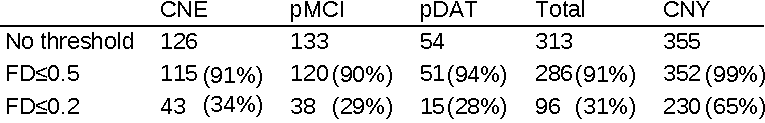
\includegraphics[width=0.75\linewidth]{../figures/table_retention.pdf}
\end{center}
\caption[Retention table after scrubbing]{
Retention rate for CNY, CNE, pMCI and pDAT at various scrubbing levels (standard, scrubbing $FD>0.5$ and scrubbing $FD >0.2$).
}
\label{tab_retention}
\end{table}

\begin{figure}[H]
\begin{center}
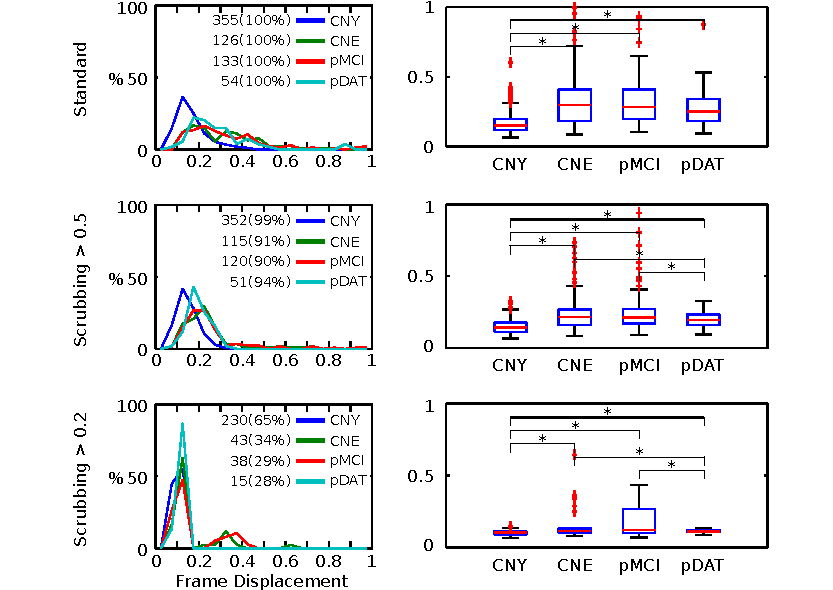
\includegraphics[width=\linewidth]{../figures/figure_fd_distrib.pdf}
\end{center}
\caption[FD distribution among groups]{
Distribution of the frame displacement (FD) for 3 groups (CNE, pMCI, pDAT) when scrubbing was applied at various levels (no scrubbing, scrubbing of $FD>0.5$ and scrubbing of $FD>0.2$). The boxplot on the right showed the distribution of FD with their associated statistical differences $t$-test (marked with a {\bf *} for a $p<0.05$).
}
\label{fig_dist}
\end{figure}

\subsection{Default mode network in young adult and elderly population}
The default-mode network (DMN) is hypothesized to be a key target of neurodegeneration in Alzheimer's disease. A visual inspection of the DMN using a standard preprocessing strategy showed more positive correlation values in the CNE population compared to the CNY (See Figure \ref{fig_avg_dmn}), probably reflecting increased partial-volume effect with cerebro-spinal fluids due to the large amount of cortical atrophy typically seen in aging. Moreover, a slight decrease in connectivity was observed in the frontal part of the DMN in the CNE population compared to the more common pattern of fronto parietal connectivity shown in the CNY population. This finding of more negative correlation for CNE subjects compared to CNY subjects was consistently observed regardless of the preprocessing strategies except for GSC, see Figure \ref{fig_avg_dmn}. The GSC seemed to increase the extent of the negative correlation found in other preprocessing strategies, as previously reported in the literature, e.g. \citep{Murphy2009}.


\begin{figure}[H]
\begin{center}
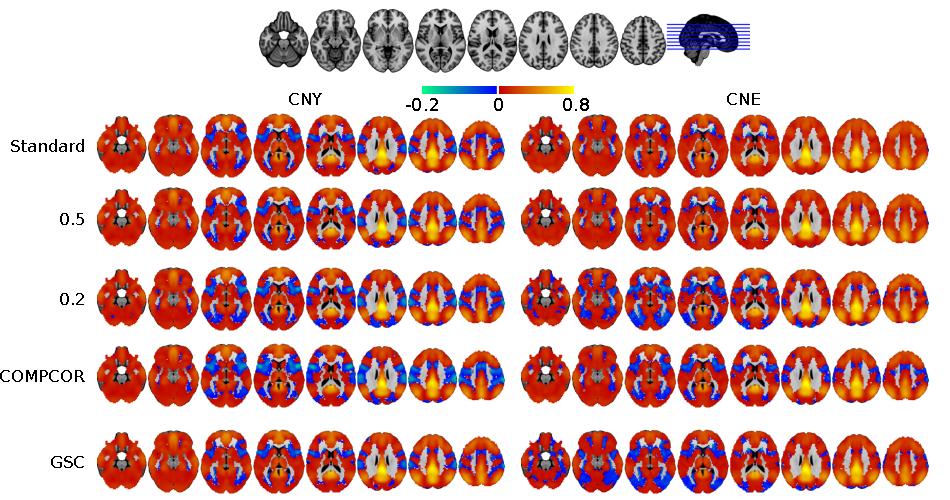
\includegraphics[width=\linewidth]{../figures/dmn_cny_cne.pdf}
\end{center}
\caption[Preprocessing impact on DMN for CNY and CNE]{ Overlay of the average default mode network (DMN) with various preprocessing strategies for CNY and CNE populations on the ICBM 152 anatomical atlas. Seed based maps with a seed in the PCC using Fisher z transform of the Pearson's r correlation between the average time series of each network.
}
\label{fig_avg_dmn}
\end{figure}

The connectivity patterns affected by scrubbing are consistent across various groups with and without dementia see Figure \ref{fig_scrubbimpact} for an example of three groups. The scrubbing procedure significantly increased connectivity strength inside the default-mode network and reduced connectivity with anti-correlated regions (Figure  \ref{fig_scrubbimpact}) consistently across all groups. More global decrease in connectivity changes can be observed for the CompCor and GSC methods. For CompCor a strong change in the sensory motor network can be observed as well as an increased connectivity in the ventral part mesio-frontal cortex. For the GSC method decreases in connectivity can be observed across the brain as well as a strong decrease in the occipital lobe.


\subsection{Impact of scrubbing on the connectivity}
\paragraph{Global impact of scrubbing}
Scrubbing significantly increased connectivity strength inside the default-mode network and reduced connectivity with anti correlated regions. Difference in functional connectivity of the DMN show significant increase of the frontal part of the DMN with scrubbing at $FD\geq0.5$ and $FD\geq0.2$ a region normally positively correlated with the PCC (see \ref{fig_scrubbimpact}). Significant decrease of connectivity with region associated with attention are also observed (dorsal attention network). The preprocessing with CompCor show massive decrease in the sensorimotor region and globally across the brain except for a mesio frontal region (anterior cingulate cortex ACC) more ventral then the expected mesio frontal region associated with the DMN (medial prefrontal cortex MPFC). The map of difference for the GSC show massive decrease in connectivity across the brain and in particular the occipital lobe, premotor and sensorimotor areas. The effect reported for the preprocessing with GSC are even more pronounced for 
the CNY group (see supplementary material Figure \ref{fig_sup_scrubbimpact_cny}).


\begin{figure}[H]
\begin{center}
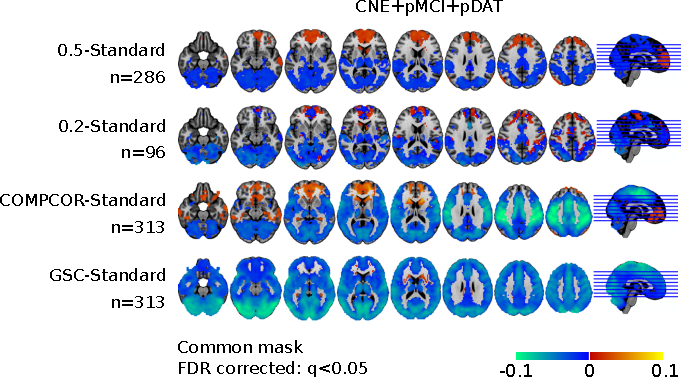
\includegraphics[width=\linewidth]{../figures/figure_comp.pdf}
\end{center}
\caption[Impact of the preprocessing on the DMN (CNE,pMCI,pDAT)]{
Differences in functional connectivity for the default mode network (seed in the PCC). Differences in connectivity between all the groups pooled together (CNE, pMCI, pDAT) with scrubbing ($FD>0.5$ and $FD>0.2$), CompCor, and GSC. The mask used depicts only significant result of the $t$-test (FDR correction $q<0.05$) only the two scrubbing procedures use the union of their respective mask (common mask).
}
\label{fig_scrubbimpact}
\end{figure}

\begin{figure}[H]
\begin{center}
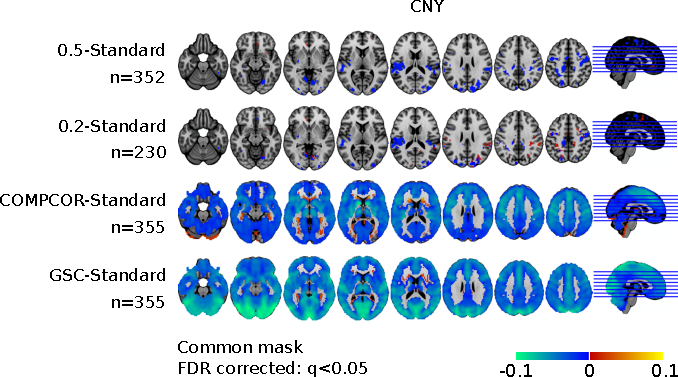
\includegraphics[width=\linewidth]{../figures/figure_comp_cny.pdf}
\end{center}
\caption[Impact of the preprocessing on the DMN (CNY)]{
{Differences in functional connectivity for the default mode network (seed in the PCC). Differences in connectivity between all the CNY with scrubbing ($FD>0.5$ and $FD>0.2$), CompCor, and GSC. The mask used depict only significant result of the $t$-test (FDR correction $q<0.05$) only the two scrubbing procedures use the union of there respective mask (common mask).}
}
\label{fig_sup_scrubbimpact_cny}
\end{figure}

\paragraph{Population specific impact of scrubbing}
The population specific difference in connectivity (see Figure \ref{fig_sup_impact_on_groups}) show almost identical findings as the combination of CNE, pMCI and pDAT therefore confirming that the observation are transferable in every population and not specific. Although the increase connectivity of the MPFC is observed in all groups when scrubbing is applied, the difference in connectivity is greater as we progress toward dementia (difference in fc for MPFC area CNE < pMCI < pDAT ). Difference map for CompCor and GSC revealed an invers patern where the greatest changes are observed in the CNE group followed by pMCI and finally pDAT for negative differences. CompCor show a increase in connectivity for the ACC area in the three groups but particularly in the pMCI group followed by CNE and then pDAT.


\begin{figure}[H]
\begin{center}
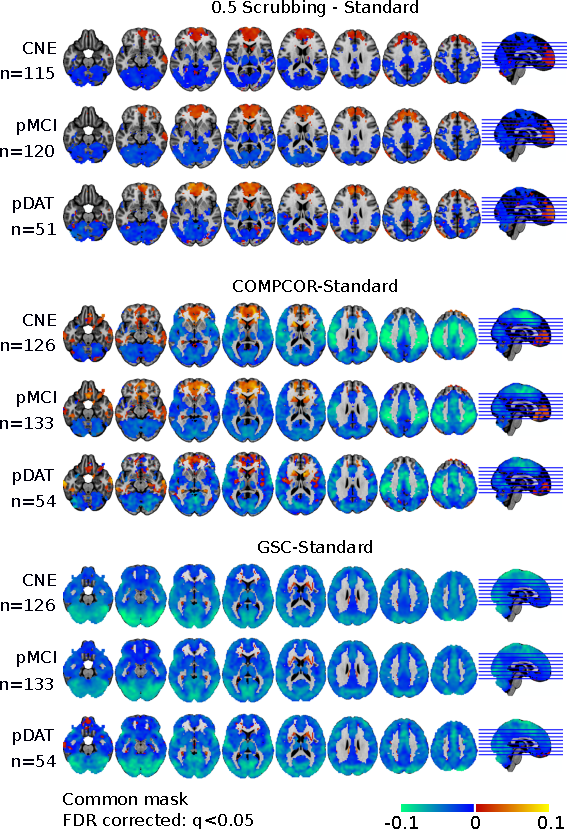
\includegraphics[width=0.75\linewidth]{../figures/scrubbing_impact_cne_mci_dat_all.pdf}
\end{center}
\caption[Impact of preprocessing on each group]{
{Differences in functional connectivity for the default mode network (seed in the PCC). Differences in connectivity for each group (CNE, pMCI, pDAT) compared to baseline (standard preprocessing) with and without scrubbing ($FD>0.5$), CompCor, and GSC (FDR correction $q<0.05$) for all voxels showing a significant effect in at least one of the contrast.}
}
\label{fig_sup_impact_on_groups}
\end{figure}

In order to assess if the significant differences in connectivity between groups are affected by the preprocessing strategy we did a $t$-test on each preprocessing strategy for every contrast (pDAT-CNE \ref{fig_impact_pDAT-CNE}, pDAT-pMCI \ref{fig_impact_pDAT-pMCI} and pMCI-CNE \ref{fig_impact_pDAT-pMCI}).

\begin{figure}[H]
\begin{center}
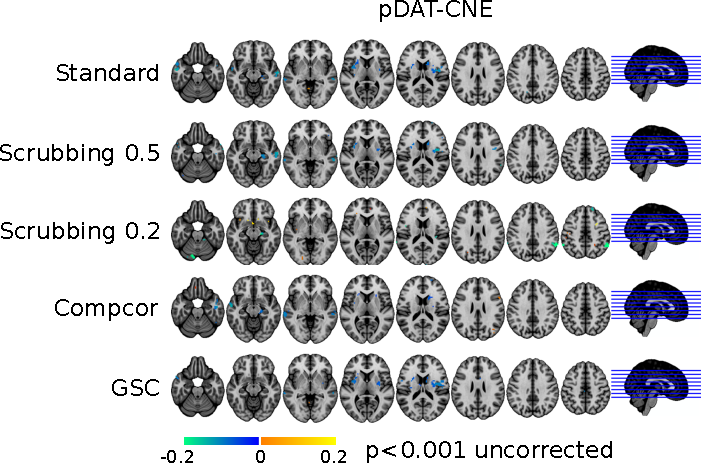
\includegraphics[width=0.60\linewidth]{../figures/scrubbing_impact_pDAT-CNE.pdf}
\end{center}
\caption[Scrubbing impact on group differences]{ Impact of preprocessing on connectivity differences between the pDAT and CNE groups. Connectivity differences between DMN ($t$-test p<0.001 uncorrected) computed with various preprocessing strategies (standard, scrubbing (0.5 and 0.2), CompCor and GSC).The maps are represented on top of the ICBM 152 anatomical atlas.
}
\label{fig_impact_pDAT-CNE}
\end{figure}

\begin{figure}[H]
\begin{center}
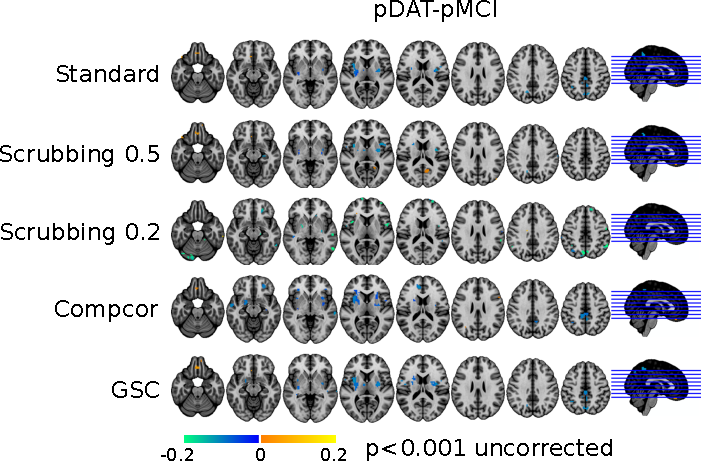
\includegraphics[width=0.60\linewidth]{../figures/scrubbing_impact_pDAT-pMCI.pdf}
\end{center}
\caption[Scrubbing impact on group differences]{ Impact of preprocessing on connectivity differences between the pDAT and pMCI groups. Connectivity differences between DMN ($t$-test p<0.001 uncorrected) computed with various preprocessing strategies (standard, scrubbing (0.5 and 0.2), CompCor and GSC).The maps are represented on top of the ICBM 152 anatomical atlas.
}
\label{fig_impact_pDAT-pMCI}
\end{figure}

\begin{figure}[H]
\begin{center}
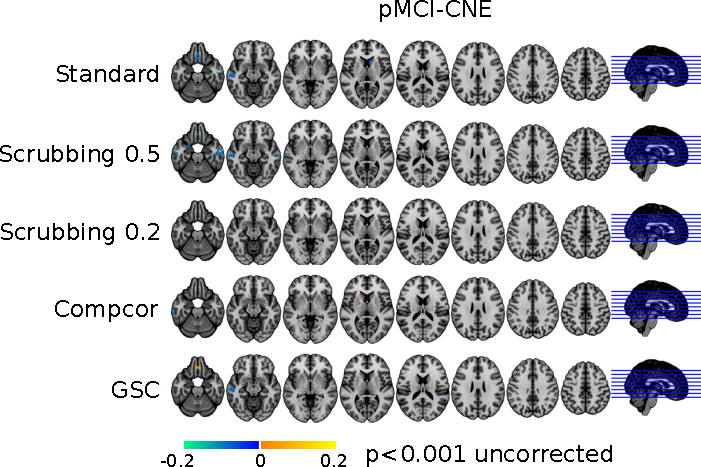
\includegraphics[width=0.60\linewidth]{../figures/scrubbing_impact_pMCI-CNE.pdf}
\end{center}
\caption[Scrubbing impact on group differences]{ Impact of preprocessing on connectivity differences between the pMCI and CNE groups. Connectivity differences between DMN ($t$-test p<0.001 uncorrected) computed with various preprocessing strategies (standard, scrubbing (0.5 and 0.2), CompCor and GSC).The maps are represented on top of the ICBM 152 anatomical atlas.
}
\label{fig_impact_pMCI-CNE}
\end{figure}


\subsection{Impact of scrubbing on our discriminative power between populations}
\paragraph{point to point connections}
Despite a moderate loss of subjects using a scrubbing at 0.5 (due to insufficient remaining data < 50 frames), the gains in data quality translated into an increased detection rate for group differences in almost all tested connections. As shown in Figure \ref{fig_p2p} the $FD\geq0.5$ scrubbing procedure mitigated motion artefacts and improved or maintain the statistical power of cross-sectional comparison of elderly clinical cohort. For $FD\geq0.2$ some improvement can be observed but the sample size remain too small to to be significant in most cases. The contrast with the most improvement due to scrubbing is the pDAT-CNE which is the contrast on which the literature point to point connections was selected for. For the pDAT-CNE contrast the most improved and consistent connections are connections with the IPL and the right SFG as well as the IPL and the dMPFC3. Connection with the PCC are also markedly improved by scrubbing namely the PCC and PCUN with MTL one of the first connection reported to be 
affected in the earliest stages of Alzheimer disease. Note that not all connection who had a good consistency with standard preprocessing improved using scrubbing. The statistical power for the pMCI-CNE contrast showed small improvements in PCC-PCUN, aMPFC-PCUN, IPL-dMPFC3 for $FD\geq0.5$ and improved consistency for SFGr-FUS with a scrubbing at $FD\geq0.2$. Finally the pDAT-pMCI contrast showed a general decrease in statistical power when scrubbing was applied, the only exception being aMPFC-PCUN that show improvement when a scrubbing at $FD\geq0.2$ was applied.

\paragraph{Detection power for every scrubbing strategy}
The simulation applied using CompCor and GSC preprocessing strategies revealed less consistency with the previously mentioned pairs of connections, especially for the pDAT-CNE contrast, that was supposed to be the optimized contrast with that selection of connection pairs. For the pMCI-CNE contrast, GSC was consistently outperformed by CompCor and Standard preprocessing in the most dominant connection, namely dMPFC-dMPFC2, PCC-PCUNm and aMPFC-MTL. On the other hand, in the last contrast pDAT-pMCI, the CompCor preprocessing was the preprocessing strategy with the most improved statistical power for aMPFC-PCUN, PCC-MTL and IPL-MTL. Interestingly, the scrubbing procedure seemed to improve the detection power more consistently and over a larger number of pair of connections than the CompCor and GSC methods (see Figure \ref{fig_p2p} and \ref{fig_sup_p2p_gsc_compcor}).


\begin{figure}[H]
\begin{center}
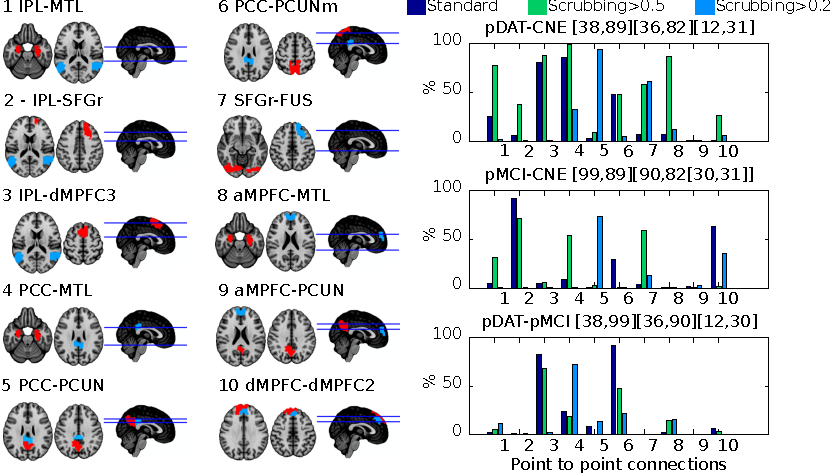
\includegraphics[width=\linewidth]{../figures/p2pdetection.pdf}
\end{center}
\caption[Detection power with Scrubbing]{
On the Left: Seeds from 10 point-to-point connections. PCC (posterior cingulate cortex), PCUN (precuneus), dMPFC (dorsomedial prefrontal cortex), dMPFC2 (dorsomedial prefrontal cortex2), IPL (inferior parietal lobule), SFGr (right superior frontal gyrus), aMPFC (anterior medial prefrontal cortex), PCUNm (precuneus motor), dMPFC3 (dorsmedial prefrontal cortex3), MTL (Mesial temporal lobe). On the right: Detection power of group differences for 3 preprocessing strategy (standard, scrubbing $FD>0.5$ and scrubbing $FD >0.2$). The detection power is computed using a $t$-test of each connection ($p<0.05$) replicated $B=10^4$ times using random subsamples of 70\% of each group. Explanatory variables included age and gender and a multi-site bias correction are applied.
}
\label{fig_p2p}
\end{figure}

\begin{figure}[H]
\begin{center}
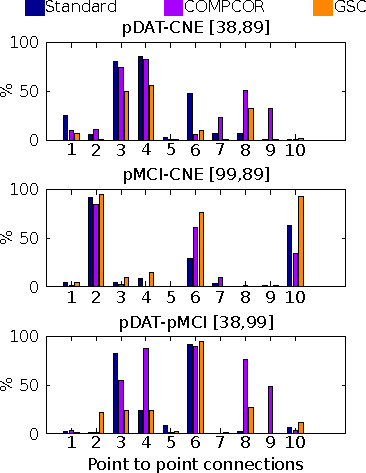
\includegraphics[width=0.5\linewidth]{../figures/p2pdetection_gsc_compcor.pdf}
\end{center}
\caption[Detection power with CompCor and GSC]{
Detection power of group differences for 3 preprocessing stategy (standard, CompCor and GSC). The detection power is computed using a $t$-test of each connection ($p<0.05$) replicated 10,000 times using random subsamples of 70\% of each group. Explanatory variables included age and gender and a multi-site bias correction are applied.
}
\label{fig_sup_p2p_gsc_compcor}
\end{figure}


\section{Conclusion} We observed that motion introduced a systematic bias in the measures of resting-state connectivity in elderly population. Populations suffering did not exhibit more severe motion level than cognitively normal elderly subjects. The scrubbing procedure mitigated motion artefacts and improved the statistical power of the detection of differences in average functional connectivity between clinical populations.
